\scanpage{38}
\margin{-- 180 --}
\margin{IX}
\uline{En d'autres termes, la filtration de} $\mathcal E^t$ \uline{induite par la filtration de Hodge} (\uline{avec les conventions de degrés} (13.4.6)) \uline{est concentrée en degré} $-1$, \uline{celle de} $\mathcal E/\mathcal E^f$ \uline{induite par la filtration de Hodge est concentrée en degré} $0$.

c) \uline{Considérons la filtration de}
\[
\mathcal E^{ab}\overset{\mathrm{dfn}}=\mathcal E^f/\mathcal E^t\simeq(\uline{\unsure{R}}^{ab})\otimes_{\mathbb Z}\uline{O}_S,\quad\text{où }\uline{R}^{ab}=\uline{R}^f/\uline{R}^t\quad(\text{cf. a)}),
\]
\figure{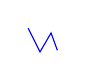
\begin{tikzpicture}\draw[blue] (0,.3)--(.15,0)--(.29,.24)--(.37,.02);\end{tikzpicture}}
\uline{induite par la filtration de Hodge de} $\mathcal E$,\uline{donc} \uline{définie par le sous-Module} $\uline{F}^{ab}$ \uline{de} $\mathcal E^{ab}$ \uline{image de}
\[
\uline{F}^f\overset{\mathrm{dfn}}=\uline{F}\cap\mathcal E^f\longrightarrow\mathcal E^{ab},
\]
\uline{(la flèche étant un monomorphisme grâce à la première relation} $(*)$).
\uline{Alors le couple} $(\uline{R}^{ab},\uline{F}^{ab}\subset\uline{R}^{ab}\otimes_{\mathbb Z}\uline{O}_S=\mathcal E^{ab})$ \uline{est isomorphe au couple} $(\uline{R}(B),\uline{F}(B))$ \uline{associé à un} groupe abéloïde \uline{sur} $S$, \uline{comme expliqué après} (13.4.4) (\uline{où donc} $B\simeq\mathcal E^{ab}/(F^{ab}+R^{ab})$, \uline{les symboles non soulignés désignant les groupes analytiques sur} $S$ \uline{correspondants}).

\uline{Remarque} 13.4.18. Dans la terminologie de DELIGNE [4], la conclusion de la proposition précédente, lorsqu'on se restreint au-dessus d'un ouvert $U$ de $S$ sur lequel $R$ est localement constant, exprime que $R$, muni des deux filtrations (13.4.17.1) de $\mathcal E=\uline{R}\otimes_{\mathbb Z}\uline{O}_S$, est une ``famille analytique de structures de Hodge mixtes sur $U$''. La situation qu'on vient d'expliciter a servie de modèle aux conjectures de DELIGNE sur la théorie de Néron en dimensions supérieures, énoncées dans [9, 9.8 à 9.13]. Il y a cependant un trait important de la théorie algébrique

\margin{498}
\fbox{498}
\mspage{37}
